%%%%%%%%%%%%%%%%%%%%%%%%%%%%%%%%%%%%%%%%%%%%%%%%%%%%%%%%%%%%
%%% ELIFE ARTICLE TEMPLATE
%%%%%%%%%%%%%%%%%%%%%%%%%%%%%%%%%%%%%%%%%%%%%%%%%%%%%%%%%%%%
%%% PREAMBLE 
\documentclass[9pt,lineno]{elife}

\usepackage[version=4]{mhchem}
\usepackage{siunitx}
\usepackage{makecell}
\usepackage[colorinlistoftodos]{todonotes} % To add todos.
\DeclareSIUnit\Molar{M}

%%%%%%%%%%%%%%%%%%%%%%%%%%%%%%%%%%%%%%%%%%%%%%%%%%%%%%%%%%%%
%%% ARTICLE SETUP
%%%%%%%%%%%%%%%%%%%%%%%%%%%%%%%%%%%%%%%%%%%%%%%%%%%%%%%%%%%%
\title{Binding thermodynamics of host-guest systems with SMIRNOFF99Frosst, an Open Force Field Group product}

\author[1]{David R. Slochower}
\author[2]{Niel M. Henriksen}
% \author[3]{Michael R. Shirts}
\author[5]{John D. Chodera}
% \author[4]{David L. Mobley}
\author[1]{Michael K. Gilson}

\affil[1]{Skaggs School of Pharmacy and Pharmaceutical Sciences, University of California, San Diego, La Jolla, CA 92093, USA}
\affil[2]{Atomwise, Inc., San Francisco, CA 94105, USA}
% \affil[3]{Department of Chemical and Biological Engineering, University of Colorado Boulder, Boulder, CO 80309}
% \affil[4]{Department of Pharmaceutical Sciences and Department of Chemistry, University of California, Irvine, CA 92697, USA}
\affil[5]{Computational and Systems Biology Program, Sloan Kettering Institute, Memorial Sloan Kettering Cancer Center, New York, NY 10065}

\corr{mgilson@ucsd.edu}{MKG}

\newif\ifdraft
\drafttrue
\ifdraft
 \newcommand{\drsnote}[1]{ {\textcolor{red} { [DRS: #1] }}}
\else
 \newcommand{\drsnote}[1]{}
\fi


%%%%%%%%%%%%%%%%%%%%%%%%%%%%%%%%%%%%%%%%%%%%%%%%%%%%%%%%%%%%
%%% ARTICLE START
%%%%%%%%%%%%%%%%%%%%%%%%%%%%%%%%%%%%%%%%%%%%%%%%%%%%%%%%%%%%

\begin{document}

\maketitle
\drsnote{I have only included authors who reviewed the outline; I'm willing to revisit this issue in the future.}

\begin{abstract}

\end{abstract}

\section{Introduction}

\section{Methods}
\subsection{Choice of host-guest systems}
In this study, we report the binding thermodynamics of 43 host-guest complexes (Figure \ref{fig:host-guest-pairs}) computed using three different force fields. 
The complexes consist of either $\alpha$- or $\beta$-cyclodextrin as host molecule and a series of ammonium, carboxylate, or cyclic alcohol small molecule guests.
The equilibrium constants and standard molar enthalpies of binding for these 43 complexes have been measured using isothermal titration calorimetry \cite{rekharsky_thermodynamic_1997} and computationally in \cite{henriksen_evaluating_2017}.
As in our previous study, only a single stereoisomer was considered for the 1-methylammonium guests.
\drsnote{Which stereoisomer was it?}

\begin{figure}[tb]
\centering
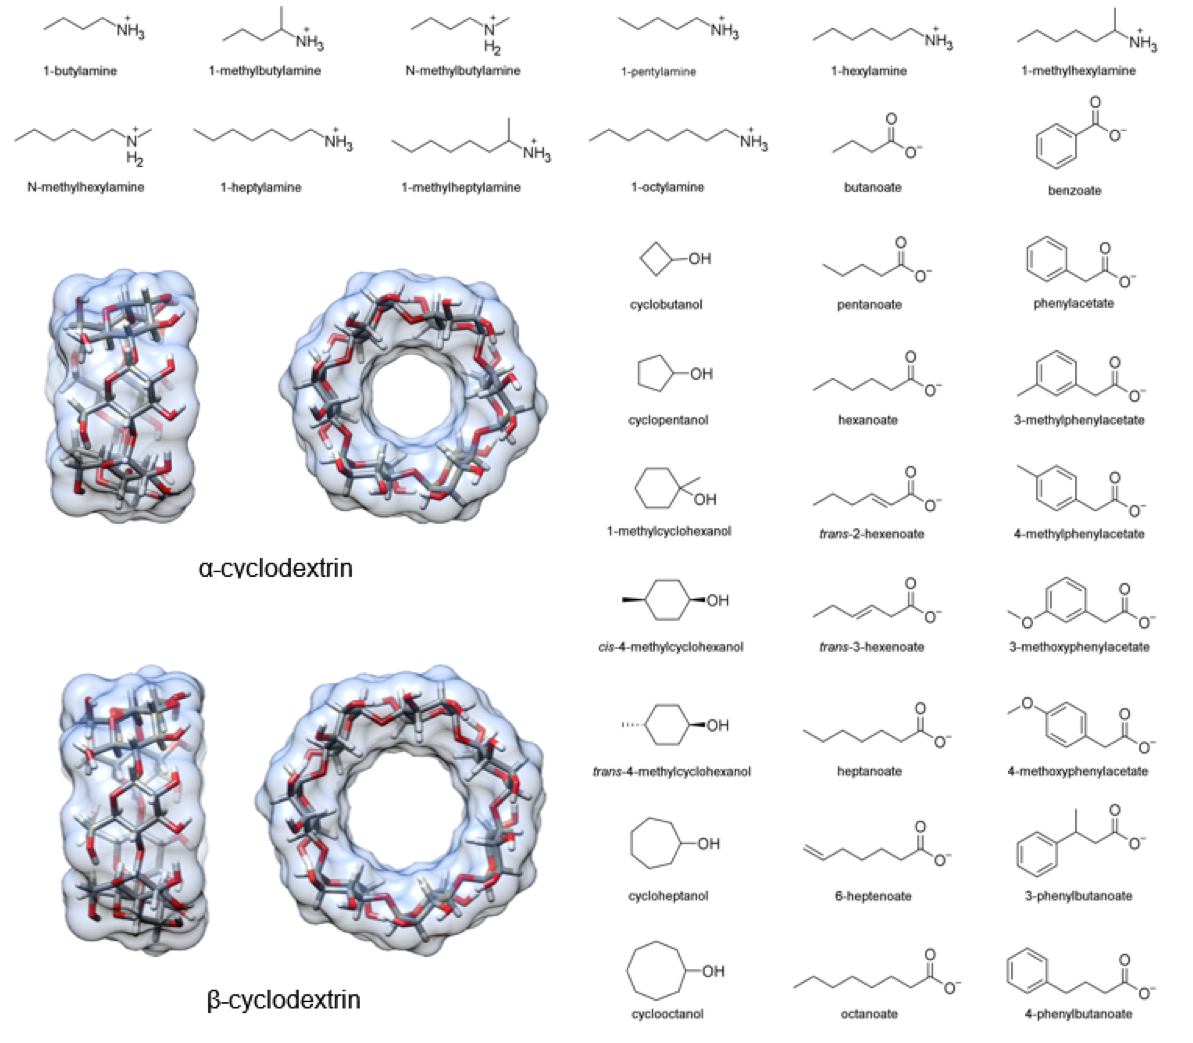
\includegraphics[width=\textwidth]{images/host-guest-pairs.png}
\caption{\drsnote{This figure is taken from Niel's paper. If I am not going to modify it, I ought to get permission for its reuse.}}
\label{fig:host-guest-pairs}
\end{figure}

\subsection{Application of force field parameters}
% Note about GAFF v1.7 parameters come from Niel's 2017 paper.
% \drsnote{How much detail do we need here, given the GAFF v1.7 parameterization scheme is well described by Niel's paper?}
\subsubsection{SMIRNOFF99Frosst}


Molecular coordinates for the 43 host-guest complexes parameterized with the GAFF v1.7 force field, AM1-BCC partial atomic charges on both host and guest molecules, and solvated with the TIP3P water model were used from our previous study \cite{henriksen_evaluating_2017}.

These calculations were performed with the Open Force Field Toolkit to version 0.0.3 and SMRINOFF99Frosst version 1.0.5.

\subsubsection{GAFF v2.1}

\subsection{Simulations}
GAFF v1.7 simulations were performed with AMBER16; GAFF v2.1 and SMIRNOFF99Frosst simulations were performed with AMBER18 molecular dynamics software.

- 2000 or 2210 waters.





\subsection{Thermodynamic calculations}
We used the attach-pull-release (APR) method as implemented in the open source package pAPRika, version 0.0.3.

A complete description of the APR method is described in \cite{henriksen_computational_2015}.

\section{Results}
SMIRNOFF99Frosst does as well as GAFF, despite far fewer numerical force field parameters.


\begin{figure}[tb]
\centering
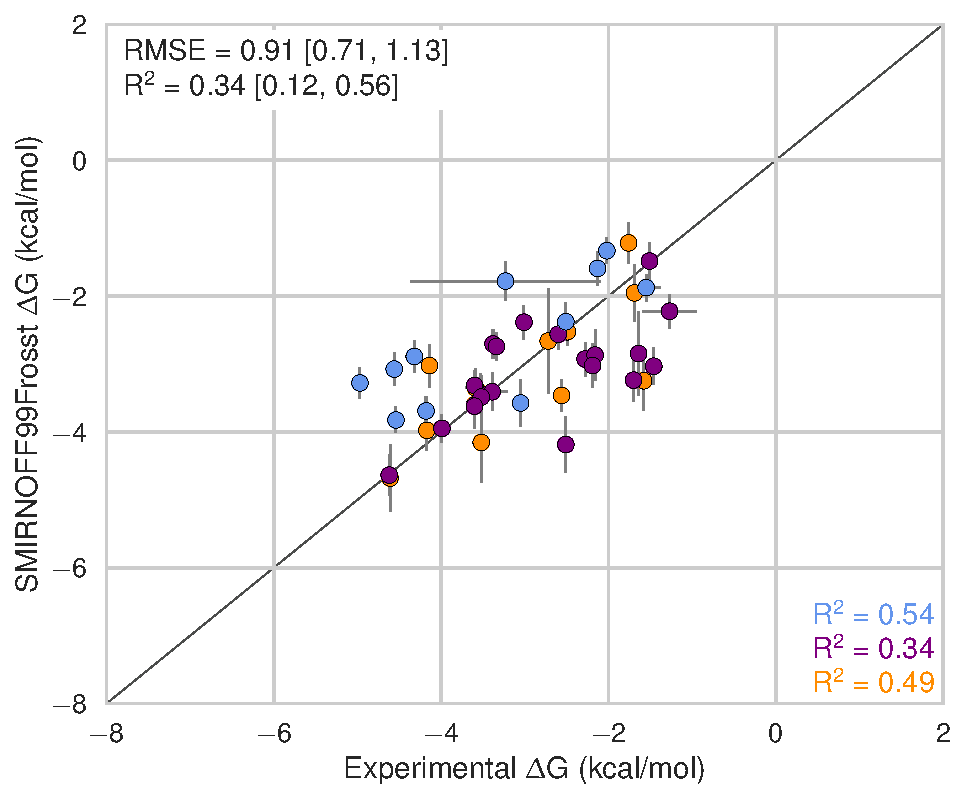
\includegraphics[width=0.49\textwidth]{images/SMIRNOFF99Frosst-vs-Experiment-dG.pdf}
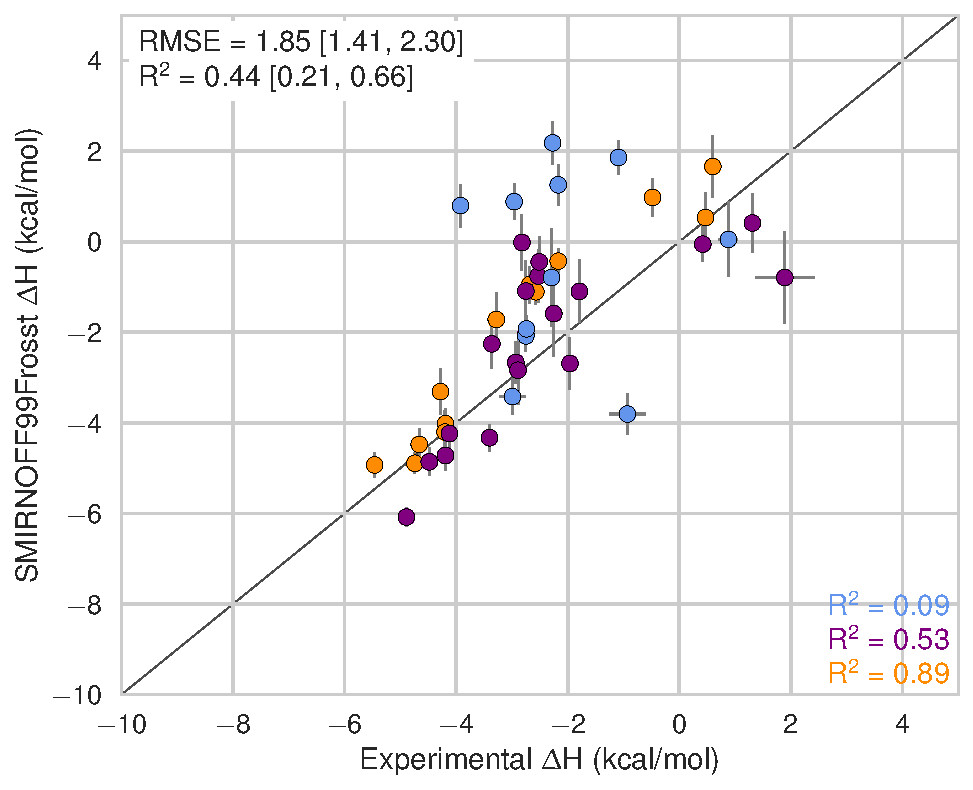
\includegraphics[width=0.49\textwidth]{images/SMIRNOFF99Frosst-vs-Experiment-dH.pdf}
\caption{Caption}
\label{fig:S99-vs-experiment}
\end{figure}

\begin{figure}[tb]
\centering
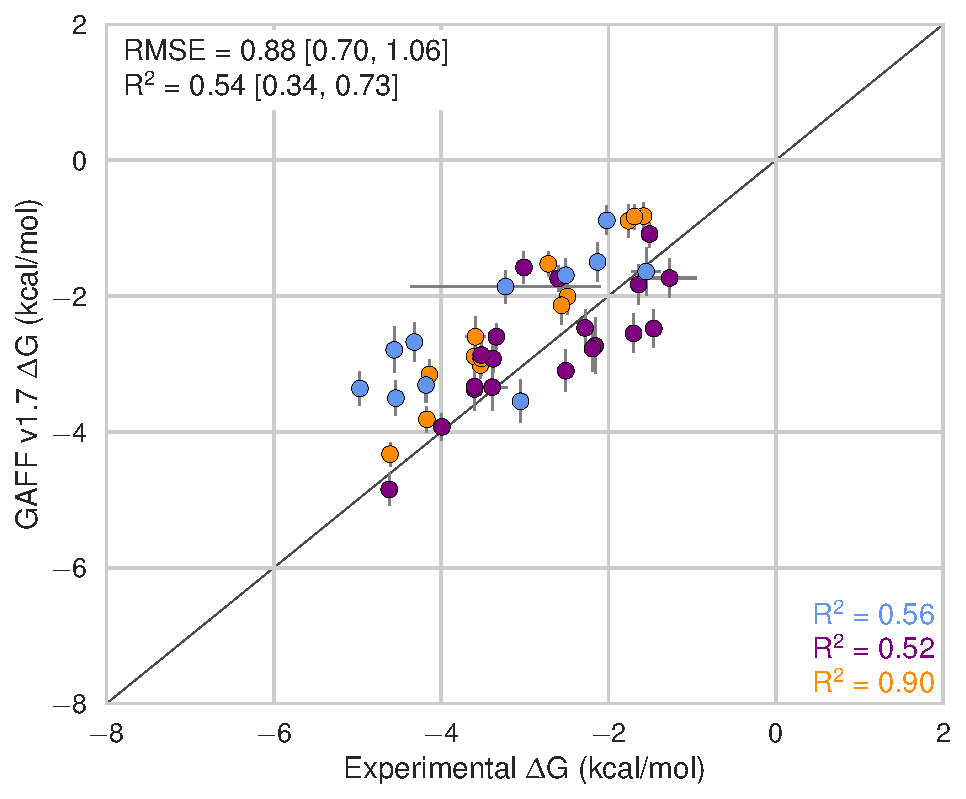
\includegraphics[width=0.49\textwidth]{{images/GAFF-v1.7-vs-Experiment-dG}.pdf}
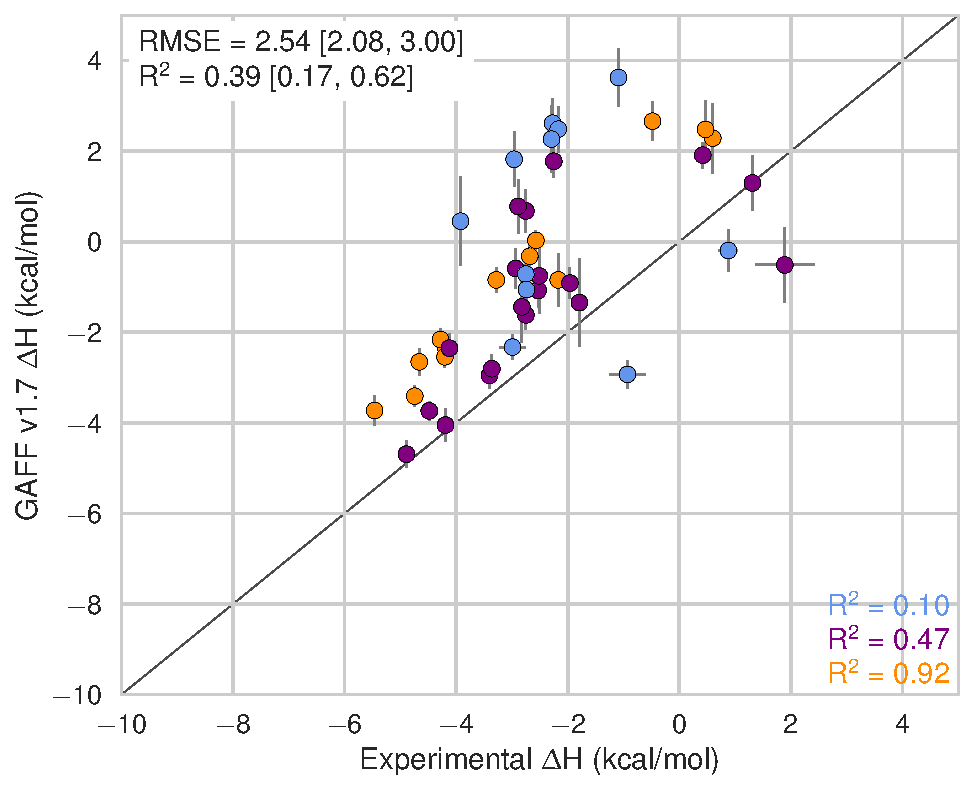
\includegraphics[width=0.49\textwidth]{{images/GAFF-v1.7-vs-Experiment-dH}.pdf}
\caption{Caption}
\label{fig:GAFF-v17-vs-experiment}
\end{figure}

\begin{figure}[tb]
\centering
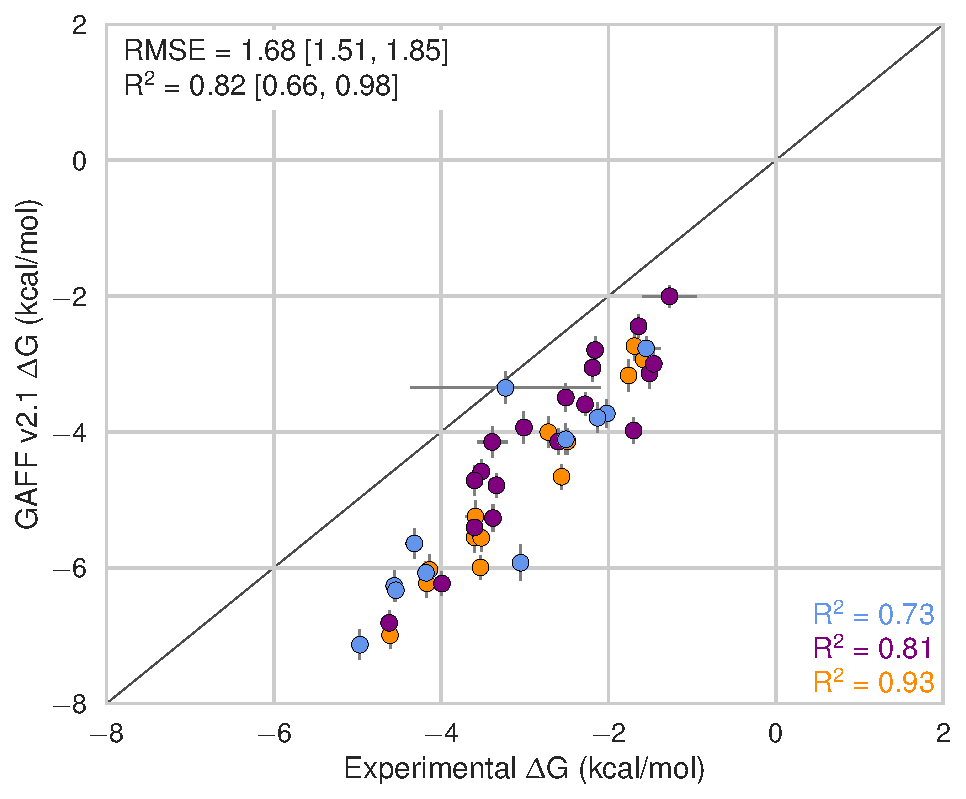
\includegraphics[width=0.49\textwidth]{{images/GAFF-v2.1-vs-Experiment-dG}.pdf}
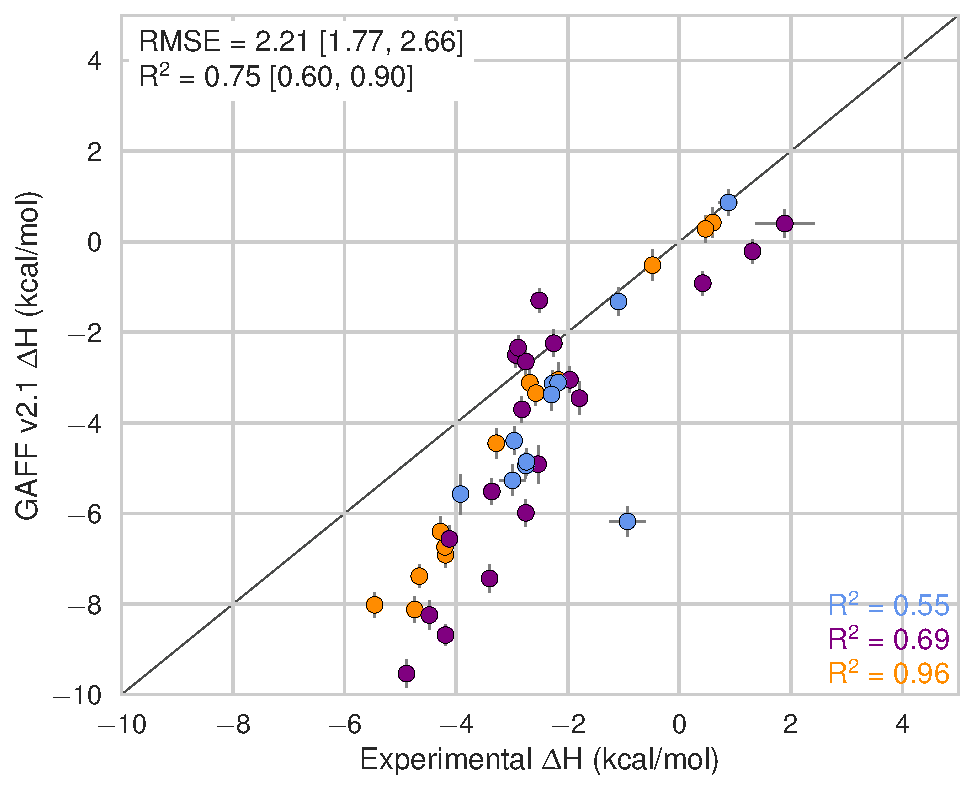
\includegraphics[width=0.49\textwidth]{{images/GAFF-v2.1-vs-Experiment-dH}.pdf}
\caption{Caption}
\label{fig:GAFF-v21-vs-experiment}
\end{figure}

\section{Discussion}

%%%%%%%%%%%%%%%%%%%%%%%%%%%%%%%%%%%%%%%%%%%%%%%%%%%%%%%%%%%%%%%%%%%%%%%%%%%%%%%%%%%%%%%%%%%%%%%%%%%%%%
% Code and Data Availability
%%%%%%%%%%%%%%%%%%%%%%%%%%%%%%%%%%%%%%%%%%%%%%%%%%%%%%%%%%%%%%%%%%%%%%%%%%%%%%%%%%%%%%%%%%%%%%%%%%%%%%

\section{Code and data availability}
\begin{itemize}
	\item Code to convert from GAFF to SMIRNOFF99Frosst
	\item Code to setup the simulations using pAPRika
	\item Code to analyze the simulation results
	\item OpenFF code and link to SMIRNOFF99Frosst
\end{itemize}
%%%%%%%%%%%%%%%%%%%%%%%%%%%%%%%%%%%%%%%%%%%%%%%%%%%%%%%%%%%%%%%%%%%%%%%%%%%%%%%%%%%%%%%%%%%%%%%%%%%%%%
% Author Contributions 
%%%%%%%%%%%%%%%%%%%%%%%%%%%%%%%%%%%%%%%%%%%%%%%%%%%%%%%%%%%%%%%%%%%%%%%%%%%%%%%%%%%%%%%%%%%%%%%%%%%%%%
\section{Author Contributions}
Conceptualization, DRS, NMH, JDC, MKG; Methodology, DRS, NMH; Software, DRS, NMH; Formal Analysis, DRS, NMH, JDC, MKG; Investigation, DRS, NMH; Resources, MKG, JDC;  Data Curation, DRS, NMH; Writing-Original Draft, DRS, NMH; Writing - Review and Editing, DRS, NMH, JDC, MKG; Visualization, DRS; Supervision, JDC, MKG; Project Administration, MKG; Funding Acquisition, MKG.

%%%%%%%%%%%%%%%%%%%%%%%%%%%%%%%%%%%%%%%%%%%%%%%%%%%%%%%%%%%%%%%%%%%%%%%%%%%%%%%%%%%%%%%%%%%%%%%%%%%%%%
% Acknowledgments 
%%%%%%%%%%%%%%%%%%%%%%%%%%%%%%%%%%%%%%%%%%%%%%%%%%%%%%%%%%%%%%%%%%%%%%%%%%%%%%%%%%%%%%%%%%%%%%%%%%%%%%
\section{Acknowledgments}
The authors declare the following competing financial interest(s): MKG has an equity interest in and is a cofounder and scientific advisor of VeraChem LLC.
%%%%%%%%%%%%%%%%%%%%%%%%%%%%%%%%%%%%%%%%%%%%%%%%%%%%%%%%%%%%%%%%%%%%%%%%%%%%%%%%%%%%%%%%%%%%%%%%%%%%%%
% Disclosures 
%%%%%%%%%%%%%%%%%%%%%%%%%%%%%%%%%%%%%%%%%%%%%%%%%%%%%%%%%%%%%%%%%%%%%%%%%%%%%%%%%%%%%%%%%%%%%%%%%%%%%%
\section{Disclosures}

\bibliography{references}

%%%%%%%%%%%%%%%%%%%%%%%%%%%%%%%%%%%%%%%%%%%%%%%%%%%%%%%%%%%%
%%% APPENDICES
%%%%%%%%%%%%%%%%%%%%%%%%%%%%%%%%%%%%%%%%%%%%%%%%%%%%%%%%%%%%

\appendix
\section{List of abbreviations}
APR, attach-pull-release
\end{document}
